\documentclass[unknownkeysallowed]{beamer}


\mode<presentation>
{
  \usetheme{Madrid}       
  \usecolortheme{default} 
  \usefonttheme{serif}    
  \setbeamertemplate{navigation symbols}{}
  \setbeamertemplate{caption}[numbered]
} 

\usepackage[english]{babel}
\usepackage[utf8x]{inputenc}
\usepackage{chemfig}
\usepackage[version=3]{mhchem}
\usepackage{graphicx}
\DeclareGraphicsExtensions{.png}





\usepackage{pgfpages}
\pgfpagesuselayout{resize to}[%
  physical paper width=8in, physical paper height=6in]


\title[Binomial trees]{Option pricing under Binomial trees}
\author{Jiang Mengjie, A. Agadzhanian and W.J. Biegstraaten}
\institute{Project group 14 \\ SFM 2016}
\date{20 July 2016}

\begin{document}

\begin{frame}
  \titlepage
\end{frame}


\begin{frame}{Outline}
  \tableofcontents
\end{frame}

\section{Introduction}
\begin{frame}{Introduction}
 This project is dedicated to the empirical assignment of Statistics of Financial Markets I Summer 2016.
\linebreak
\linebreak
Case:
"Check the Quantlet of the Binomial tree, and apply to the options of any kind, and make a comparison with the market data." 
\linebreak
\linebreak
(Note: You need to check the data availability of the option you choose.)

\end{frame}

\subsection{Description}
\begin{frame}{Description}
Abstract:
\begin{block}{}
To begin we use the CSI 300 Index option under various strikes ranging from 1.8 till 2.25. The price of the underlying (S0) is 2,136.  We take different time to maturities as in options expiring in August, September and December; To check for differences between time periods. The time to maturity is set at yearly rate. We compute both the call(1) and put(0) options as binary value. We take volatility at an annual rate which in this case is 0,1323 and a annual interest rate of 0.0305. We've extracted the data from the Wind System and therefore use those numbers from the option of the market as the parameters manually. We then compute the Binomial tree in a 5 step model to estimate option pricings under European options. In the end we compare prices from the market data with those calculated by the Binomial tree to make up a conclusion.
\end{block}

\end{frame}

\section{The Binomial Model for European option: an application with Chinese option}
\subsection{Empirical results}

\begin{frame}
\frametitle{The Binomial Model for European options: on CSI 300 Index option}
Result stock price tree (no dividend):
\vskip 0.10cm
\begin{figure}[]
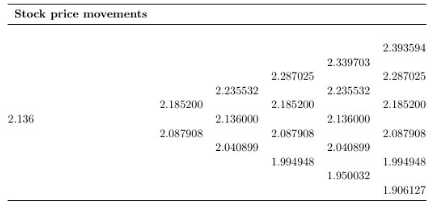
\includegraphics[scale=1]{stock_price_tree}
\end{figure}
\end{frame}

\begin{frame}
\frametitle{The Binomial Model for European options: on CSI 300 Index option}
Result Option price tree (no dividend):
\vskip 0.10cm
\begin{figure}[]
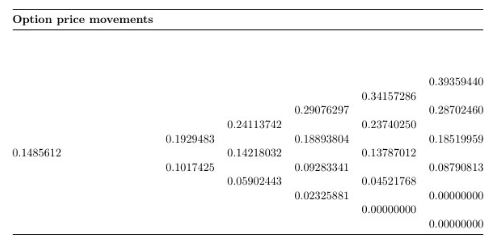
\includegraphics[scale=0.9]{option_price_tree}
\end{figure}
\end{frame}


\section{Conclusion}
\begin{frame}{Conclusion (1/2)}
We conclude that the CSI 300 Index options are mispriced. During 2016, specifically the researched months August and September -and October, the theoretical price and market price differ, the reasons are listed as following:
\linebreak

 \begin{itemize}
    \item{In practice stock option prices fluctuate around their theoretical price. The market sentiment may influence option prices a lot, thus be affected by  supply and demand. In the bull market, option prices may be higher, in bear market they usually are lower. As we all know in the last year china’s stock market has experienced great fluctuation during July and August, after that  it has turned from bull-market to bear-market. The market environment has changed a lot, so the stock prices and option prices may be affected by extreme emotion in the market.}
     \end{itemize}
\end{frame}

\begin{frame}{Conclusion (2/2)}
 \begin{itemize}
 \item{Because of stock market’s crash in the last year, China Securities Regulatory Commission has banned most part of stock price option trading. Therefore the trading is limited, so the market can’t work properly, causing option prices to deviate.}
 \linebreak
    \item{In an ideal model parameters such as risk-free interest rate are constant, but actually it is time-varying. The Chinese government adjusts currency policies causing the risk free rate to change, but in our model it doesn’t adjust accordingly.}
    \end{itemize}
    \end{frame}
\end{document}